%%%%%%%%%%%%%%%%%%%%%%%%%%%%%%%%%%%%%%%%%%%%%%%%%%%%%%%%%%%%%%%%%%%%%%%%%%%%%%%%
\subsection{Interactions Between Photons \& Rydberg Atoms}

Photons don't interact with each other in free space, which posses a problem if we want to create logical gates with qubits using optical light. In order to have strong and coherent interactions between photons, it's possible to use an intermediary material thanks to non-linearity of light-matter interaction. In effect, atomic resonances are unequally spaced in frequency. As a result, if one atom absorbs a photon, it will not be able to absorb a second identical one without a re-emission. This second photon arriving just after a photon absorption will experience a much higher potential compared to the first photon. Intuitively, we can have a single atom or molecule in free space and shoot photons at it, which unfortunately yields a low probability of absorption and random directions of spontaneous emission. This implies that the information about the emitted photon is lost, which is undesirable if we want to create a quantum logic gate having the property of reversibility.

To circumvent such undesired effects, the Quantum Photonics team in which I did my internship chose to use a cloud assembly of $N$ Rubidium 87 atoms coupled to Rydberg states that is confined within a cavity of medium finesse. A cavity confinement gives control over the direction of photon re-emission, and the Rydberg state introduces non-linearity that prevents the absorption of a second photon. A very fine cavity increases the probability of absorption, but introduces problems related to the quality of the mirrors and to the size of the beam. Thus a cloud assembly of $N$ atoms for which the coupling is multiplied by $\sqrt{N}$ was preferred as it permitted a larger cavity with medium finesse, making the experiment more swiftly repeatable.

Rydberg atoms are atoms with excited quantum states close to ionization, i.e. with principal quantum number $n \gg 1$. In this experiment, $^{87}$Rb atoms are excited towards spherical states $nS_{1/2}$ with $n \sim 100$. A probe beam transitions the $5^2S_{1/2}$ state to the $5^2P_{1/2}$ state, and then a control beam transitions the $5^2P$ state to the Rydberg $nS_{1/2}$ state.

The low overlap between the ground state and excited state wavefunctions gives Rydberg states a very long lifetime and very narrow linewidth. A Rydberg excitation in the atom cloud leads to strong Van der Waals interactions with other atoms, contributing to high polarizabilities, such that no other Rydberg excitation can occur within a ``blockade" sphere of radius $R_\text{b}$ around the Rydberg atom. This Rydberg ``blockade" phenomenon is illustrated in Figure \ref{fig:ch1_blockade_sphere}. The experimental parameters used in the lab results in $R_\text{b} \simeq 15\ \mu\text{m}$ to $20\ \mu\text{m}$, while the density of the atomic cloud has a Gaussian standard deviation of $5\ \mu\text{m}$. This signifies that only one Rydberg excitation can exist within the atom cloud under our experimental conditions.

\begin{figure}[ht]
    \centering
    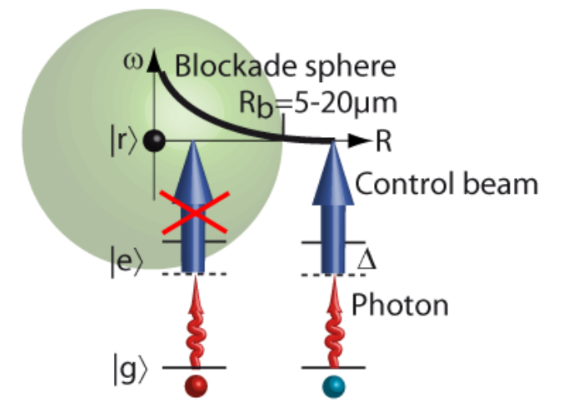
\includegraphics[width=0.4\columnwidth]{images/chapter_1/blockade_sphere.png}
    \caption{Schematic diagram of the Rydberg blockade effect. The Van der Waals dipole interaction of an existing Rydberg excitation prevents a second photon from being resonant within a blockade radius $R_\text{b}$ around the first excitation. If the atom cloud is smaller than $R_\text{b}$, then only one Rydberg excitation can exist within the entire cloud.}
    \label{fig:ch1_blockade_sphere}
\end{figure}

%%%%%%%%%%%%%%%%%%%%%%%%%%%%%%%%%%%%%%%%%%%%%%%%%%%%%%%%%%%%%%%%%%%%%%%%%%%%%%%%
\subsection{Experimental Setup}

The entire experimental setup is very involved and sizable, and is divided into three parts. One part is used to control the different lasers, a second part prepares the different laser beams, and a third part houses the vacuum chamber in which the Rubidium atoms are prepared. A section of the first two parts is shown in Figure \ref{fig:ch1_lenses} and the vacuum chamber is shown in Figure \ref{fig:ch1_cavity}.

The experimental setup already somewhat reveals that the start-to-end process of the experiment -- from laser preparation, atomic cloud preparation, to Rydberg excitation via controlled laser behavior, etc. -- involves many calculated steps. Therefore, the experiment requires various digital and analog I/O modules and numerous respective I/O channels that send and receive instruction, signals, and data samples for experimental monitoring and processing. As a consequence, a smart and efficient data acquisition (DAQ) mechanism becomes crucial.

\begin{figure}[ht]
    \centering
    \begin{subfigure}[t]{0.48\linewidth}
        \centering
        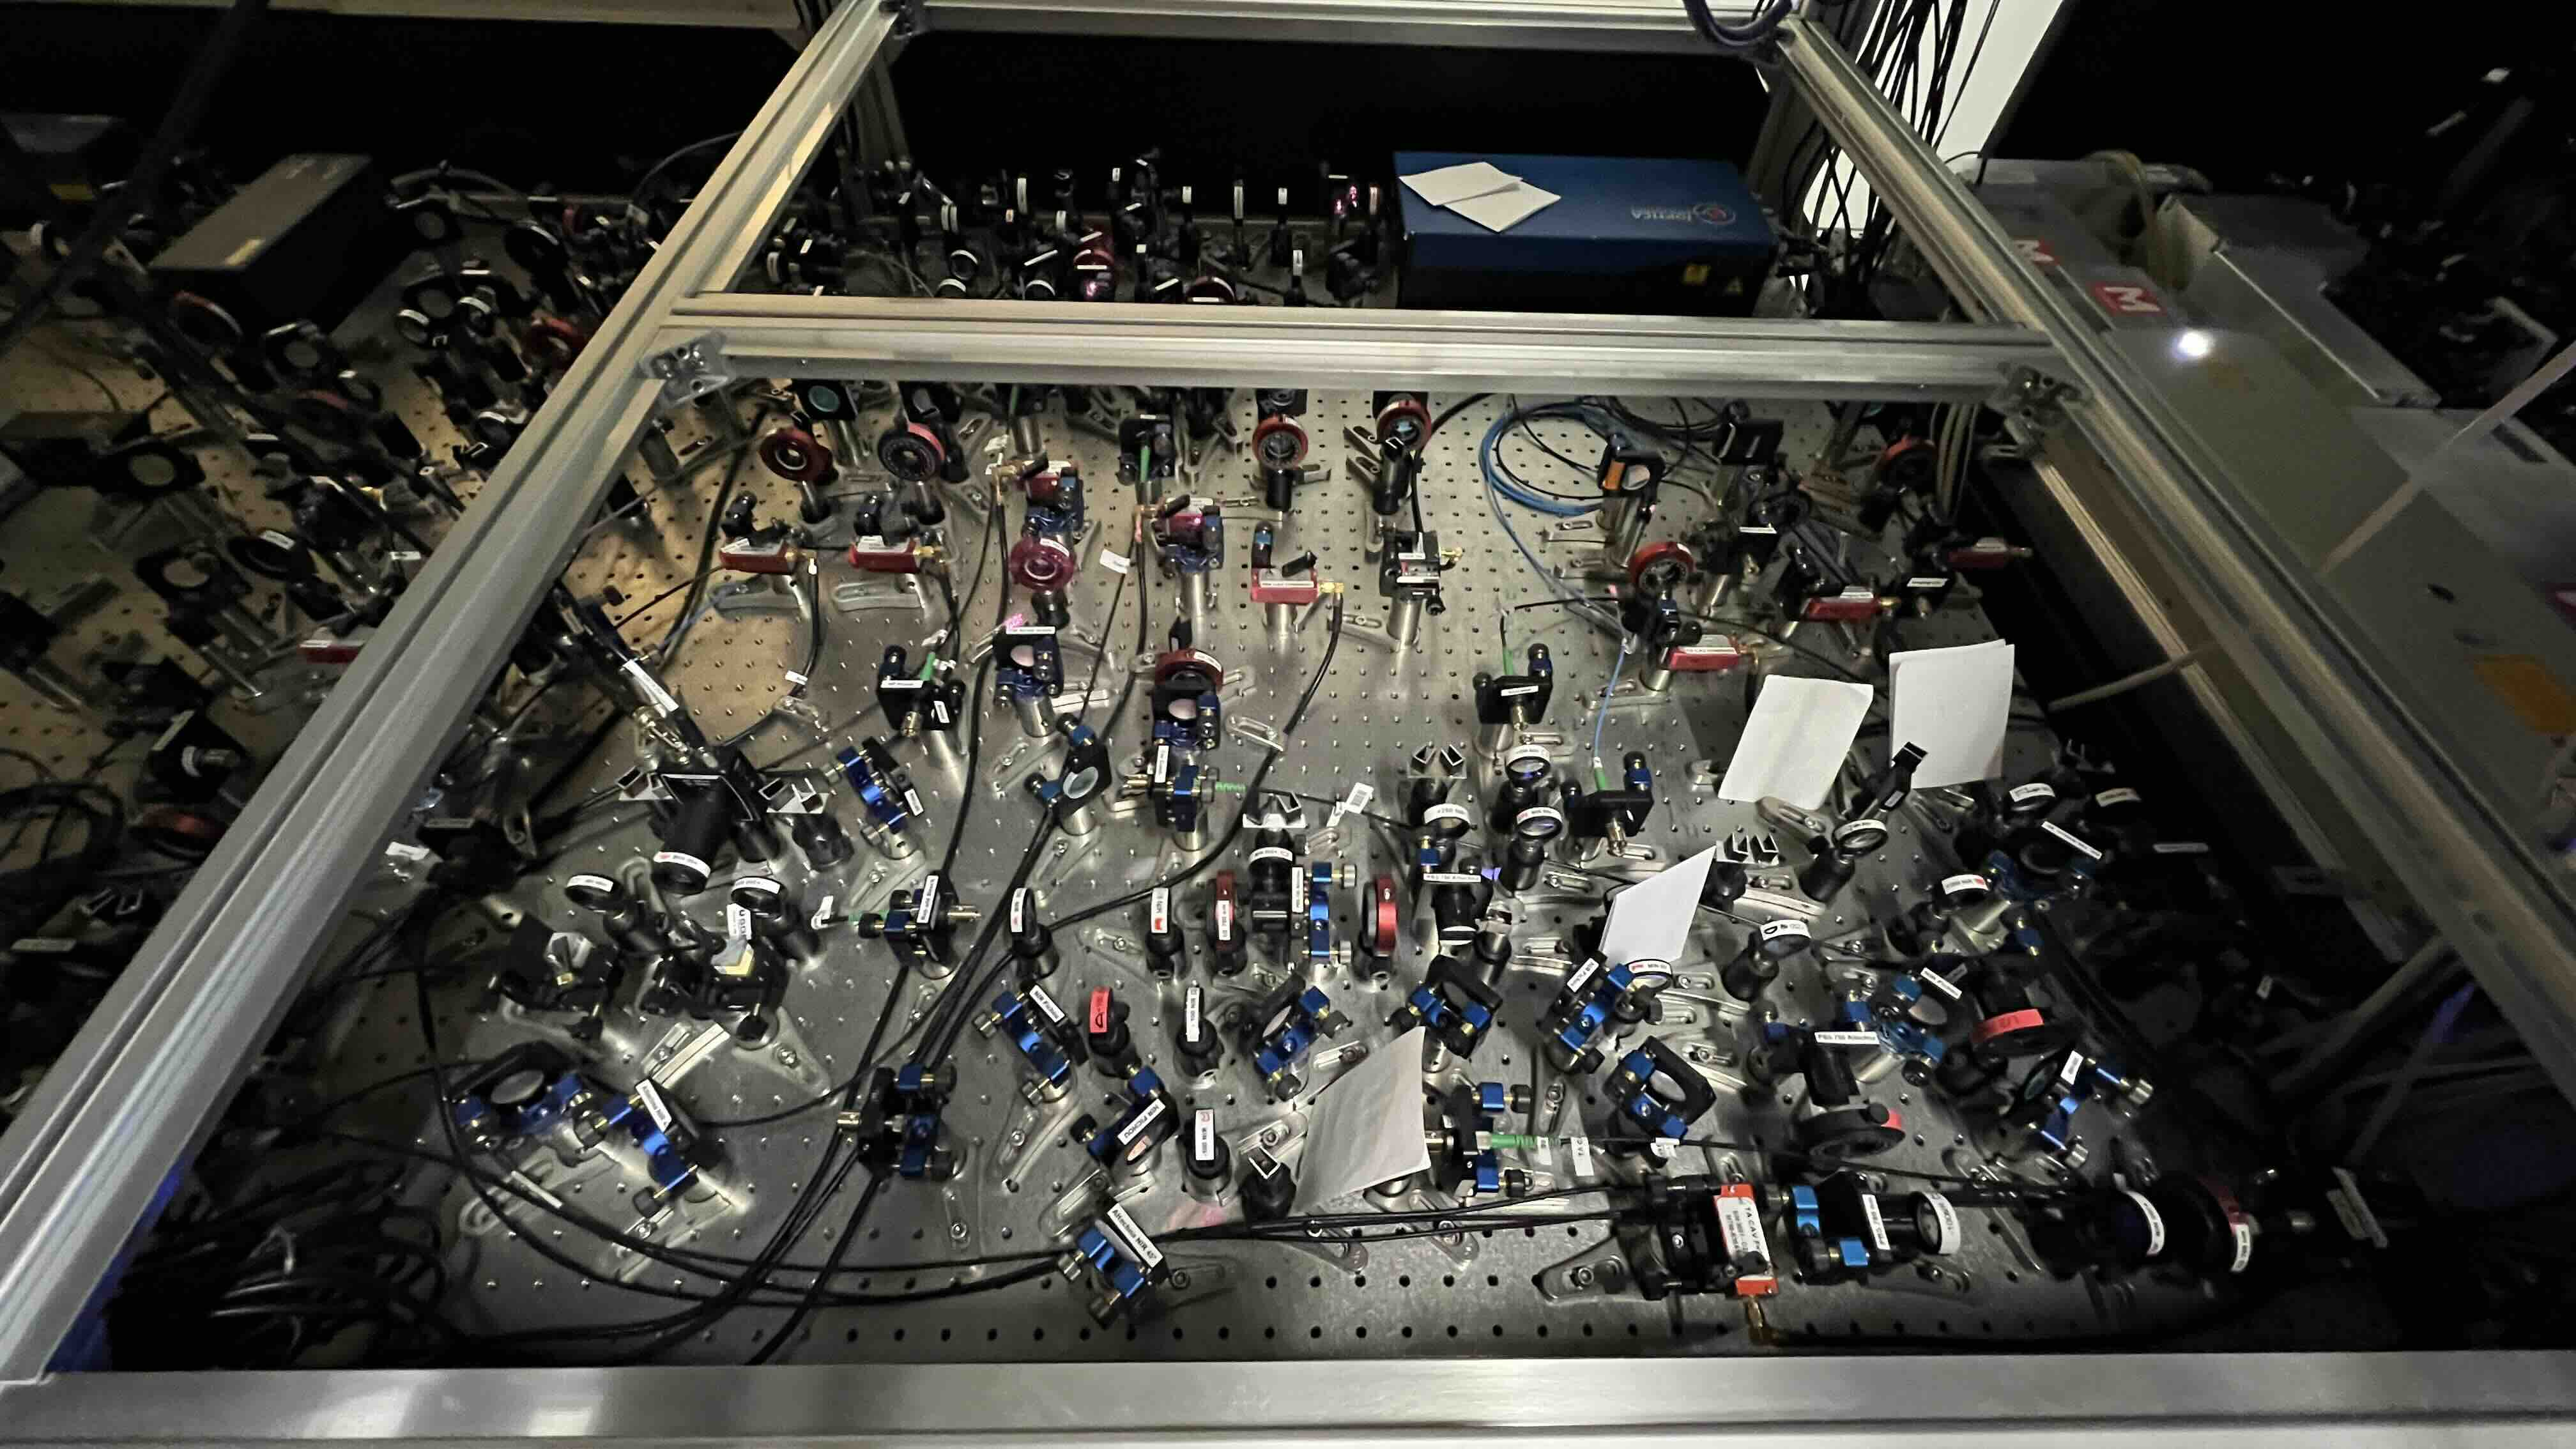
\includegraphics[width=\textwidth]{images/chapter_1/lenses.jpg}
        \caption{Various physical devices used to control laser beams.}
        \label{fig:ch1_lenses}
    \end{subfigure}
    \hspace{.025\linewidth}
    \begin{subfigure}[t]{0.48\linewidth}
        \centering
        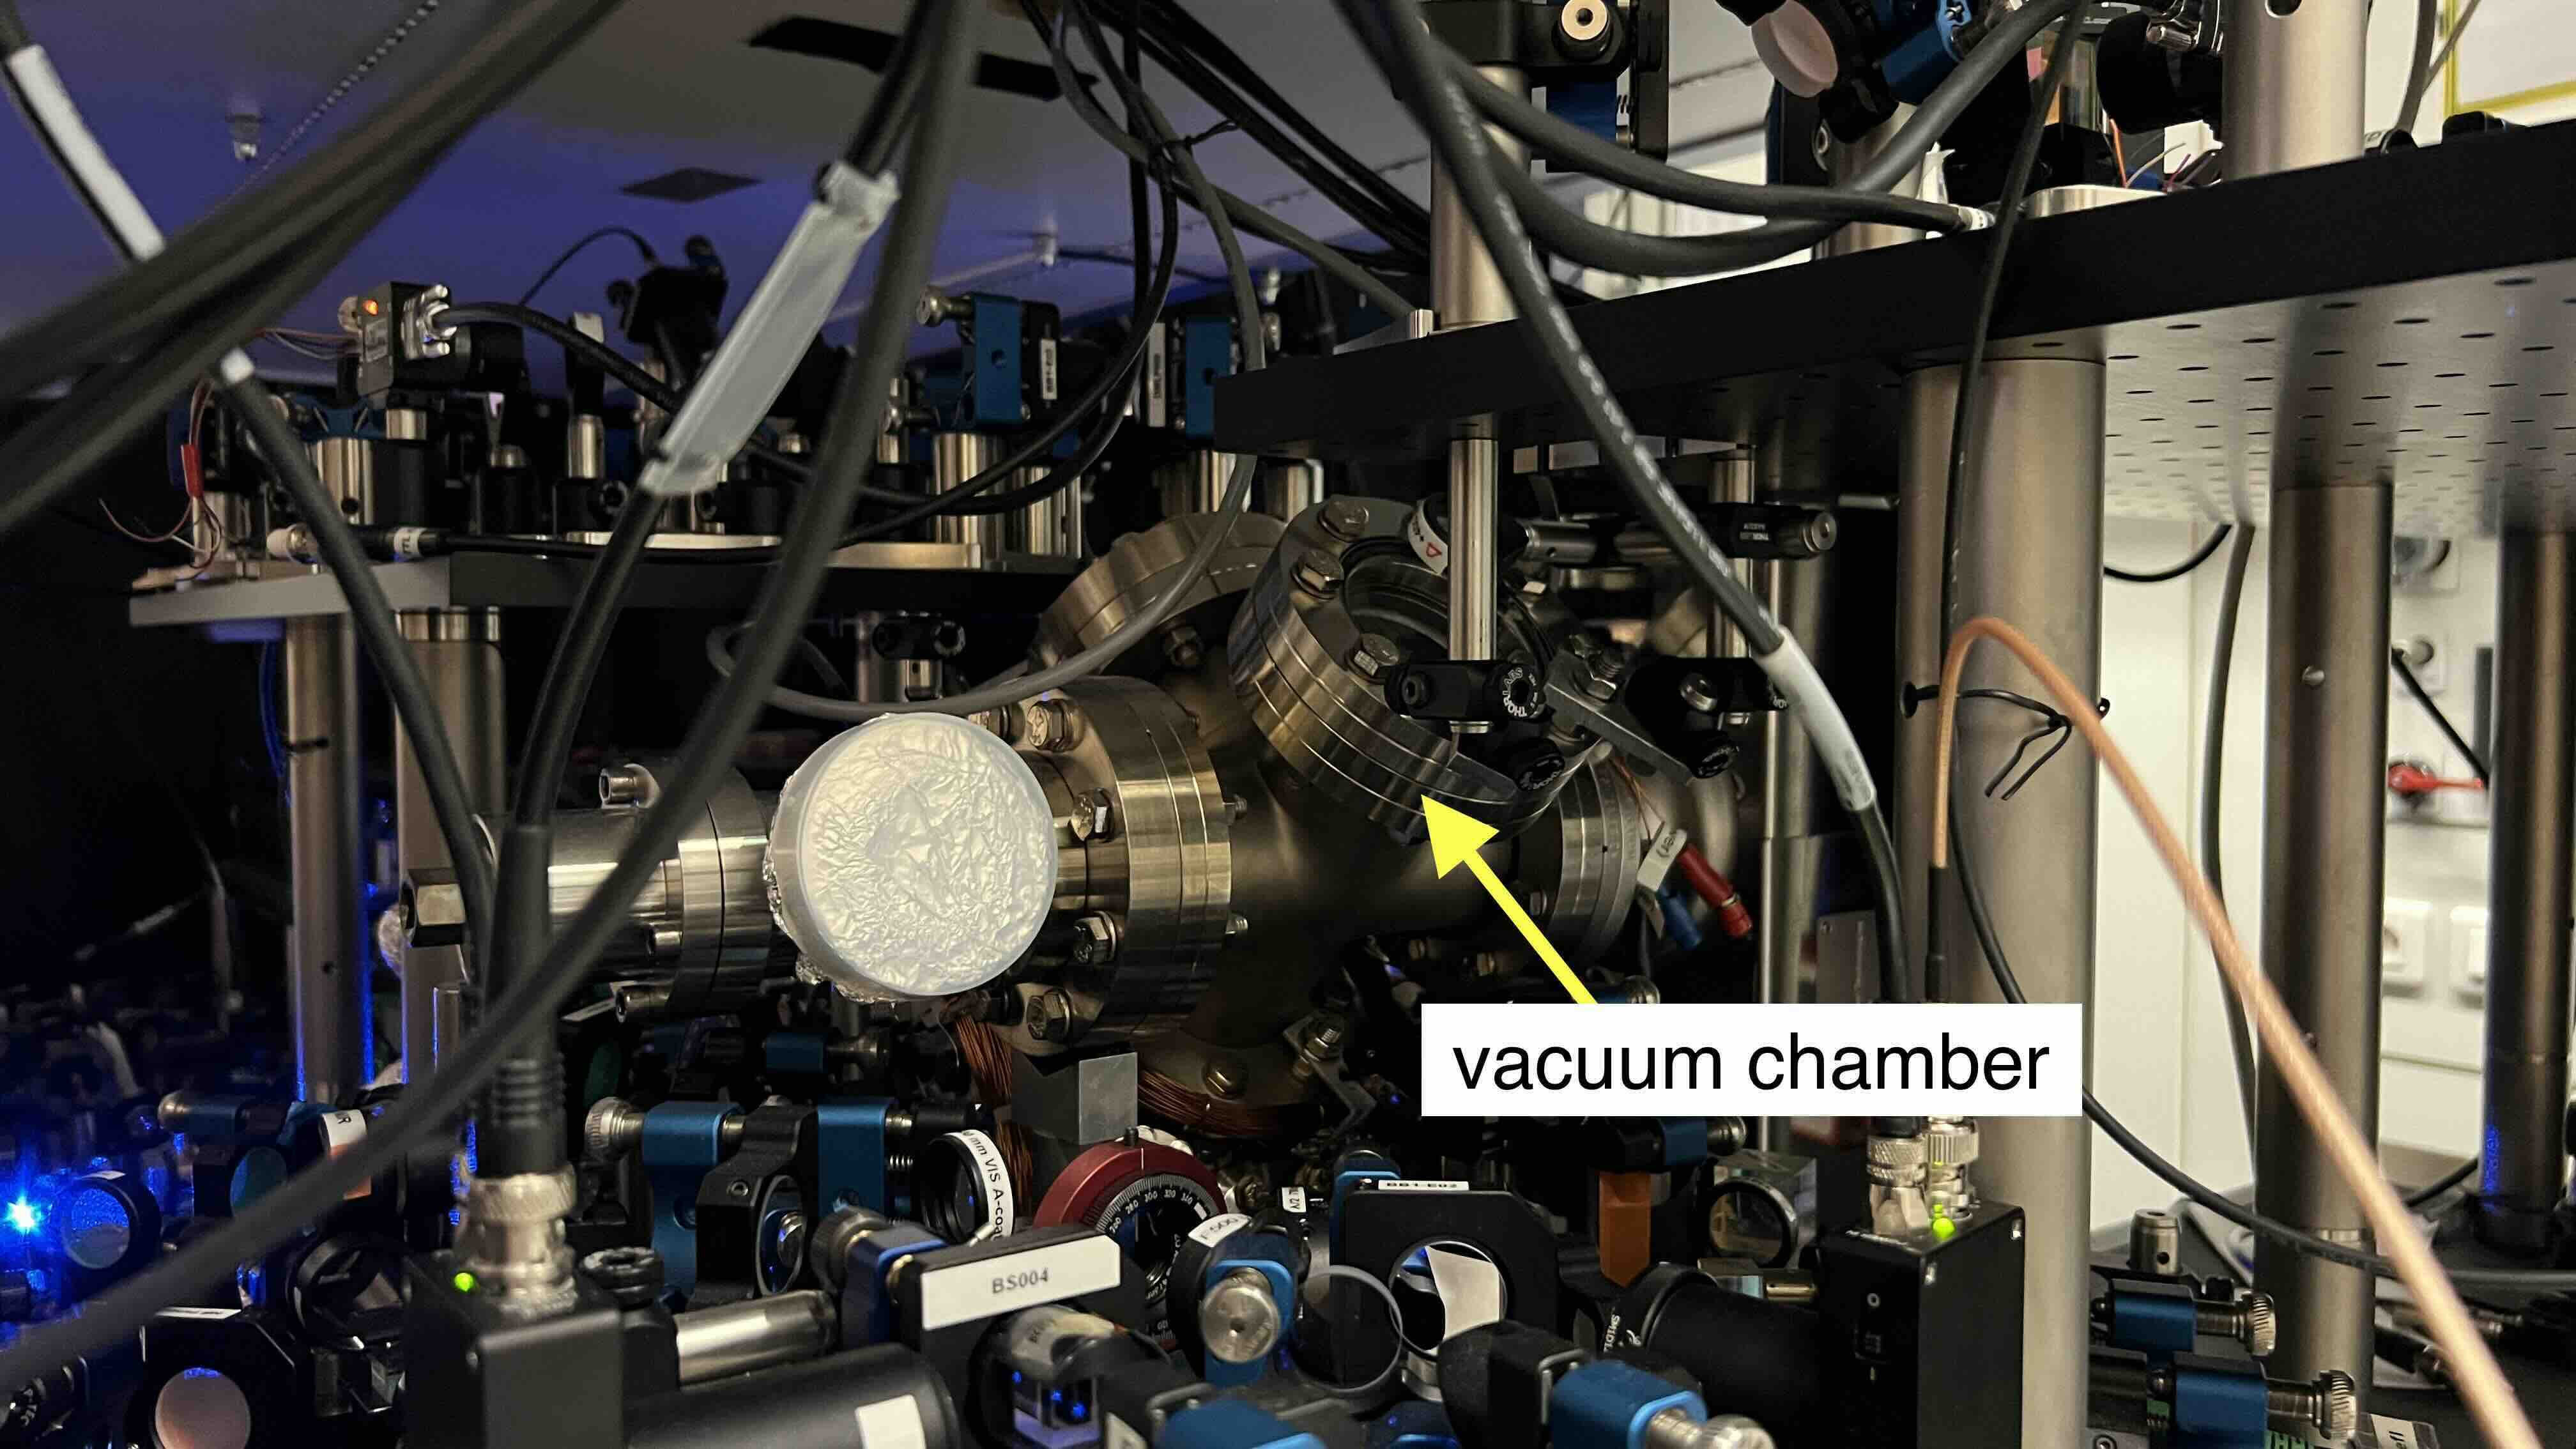
\includegraphics[width=\textwidth]{images/chapter_1/cavity.jpeg}
        \caption{A fraction of the vacuum chamber that hosts the optical cavity, in which the Rb atom cloud is confined and prepared.}
        \label{fig:ch1_cavity}
    \end{subfigure}
    \caption{Experimental setup.}
    \label{fig:ch1_exp_setup}
\end{figure}